
%
%%%%%%%%%%%%%%%%%%%%%
% Special Instructions
%%%%%%%%%%%%%%%%%%%%%
%
% Please follow these instructions to use line numbering package (lineno.sty):
%
%   http://fourforces.wordpress.com/2008/04/24/add-line-numbers-using-linenosty-in-revtex-4/
%

\RequirePackage{lineno}

\documentclass[aps,prc,twocolumn,groupedaddress,showpacs,amsmath,amssymb,floatfix,superscriptaddress]{revtex4}
\usepackage{multirow}
\usepackage{graphicx}
\usepackage{times}
\usepackage{textcomp}

\bibliographystyle{apsrev}


\usepackage{color}

\newcommand{\nuebar}{$\overline{\nu}_{e}$}
\newcommand{\PerTonDay}{(ton$\cdot$day)$^{-1}$}
\hyphenation{KamLAND}

\begin{document}

\bibliographystyle{h-physrev3}

\title{Directionality in Kilo-ton Scale Scintillating Neutrino Detectors}

% All university affiliations addresses go here:
\newcommand{\ucla}{\affiliation{University of California Los Angeles, Los Angeles, CA 90049, USA}}
\newcommand{\chicago}{\affiliation{University of Chicago, Chicago, IL, XXXX, USA}}

%
\author{C.~Aberle}\ucla
\author{A.~Elagin}\chicago
\author{L.~Winslow}\ucla

\date{\today}

\begin{abstract}
Liquid scintillator detectors are some of the most prevalent detectors due to their good energy resolution and scalability to large volumes. This has made them particularly attractive for neutrino measurements, and this technology is at the heart of many of the most important measurements in this field. Their weakness is that they only provide information on the energy of the particle. The extraction of a second signal like the particle direction would greatly enhance the scientific reach of these detectors especially for searches for neutrinoless double-beta decay. In this paper, we develop a technique for extracting particle direction and evaluate different detector advances that could be used to make direction reconstruction a reality in a kilo-ton scale detector.
\end{abstract}

\pacs{23.40.$-$s, 21.10.Tg, 14.60.Pq, 27.60.$+$j}

\maketitle

\section{Introduction}
Liquid scintillator based detectors are responsible for several of the critical measurements that have cemented our understanding of three-neutrino oscillations. These measurements include KamLAND's measurement reactor antineutrino oscillation at a distance of $\sim$200~km, Borexino's measurement of $^{7}$Be solar neutrino oscillation and most recently the short baseline reactor antineutrino experiments that measured oscillations due to $\theta_{13}$ at a distance of 1~km: Daya Bay, Double Chooz, and RENO.  Scintillating neutrino detectors will continue to be important  for the next set of neutrino measurements from the determination of the neutrino mass hierarchy to elastic scattering measurements and sterile neutrino searches and for non-proliferation applications. Their scalability to large volumes makes them particularly attractive for neutrinoless double-beta ($0\nu\beta\beta$) decay searches, and currently one of the best limits for the $0\nu\beta\beta$ half-life comes from KamLAND-Zen.

The advantage of liquid scintillators for measurements in the $\sim$1~MeV range is their simple scalability from  1~ton to 1~kiloton while providing energy resolutions of $\sim$5\%. This is roughly a factor of two better than water Cerenkov detectors, the other technology that is easily scaled to these  large masses. While the energy resolution is good due to the abundant scintillation light, this light is isotropic and does not retain the directional information of the primary particle.   In contrast, the direction of the particle can be reconstructed from the Cerenkov cones in water-based detectors, but the energy resolution rapidly degrades below $\sim$5~MeV.

In a scintillating detector, Cerenkov light is produced although most is absorbed and reemitted as part of the scintillation processes; however, some fraction retains its directional information. If this directional Cerenkov light can be isolated from the copious isotropic scintillation light then it may be possible to reconstruct the direction of the primary particle or at least determine something about the topography of the event. The addition of directionality is a powerful tool for background rejection and could be used to search for new physics especially in the case that $0\nu\beta\beta$ is observed. In this paper, we develop a technique for separating the Cerenkov and scintillation using the photon arrival times and evaluate different detector technologies that would allow the realization direction reconstruction in kilo-ton scale scintillating neutrino detectors.


\section{Light Production in Liquid Scintillators}
Molecules vibrate...index of refraction = Cerenkov.

\section{Geant4 Simulation}
In order to study the effects relevant to directionality reconstruction in liquid scintillators, a Geant4 \cite{geant4one,geant4two} simulation has been set up. The presented simulation application has been developed using standard Geant4 functionality for the optical model of the liquid scintillator. Version Geant4.9.6 is used and the simulation appliction has been built from a customized official application examples. The simulation is kept simple to provide generally applicable information about the main factors in directionality reconstruction. 

The implemented detector geometry is a sphere of 6.5~m (or 0.65~m) diameter filled with liquid scintillator. The scintillator properties have been chosen to match the KamLAND scintillator as the default simulation settings \cite{tbd}: 80~\% n-Dodecane, 20~\% Pseudocumene (1,2,4-Trimethylbenzene) and 1.52~g/l PPO (2,5-Diphenyloxazole). The implemented scintillator properties include the atomic composition and density ($\rho$ = 0.7752~g/ml), the wavelength-dependent attenuation length and refractive index, the scintillation emission spectrum, emission rise time ($\tau_r$ = 1.0~ns) and emission decay time constants ($\tau_{d1}$ = 6.9~ns and $\tau_{d2}$ = 8.8~ns with relative weights of 0.87 and 0.13), scintillator light yield (LY, 9030.5 photons/MeV) and the Birks constant ($kB$ = 0.106~mm/MeV) \cite{tbd}. Variations from the baseline KamLAND case are discussed below when applicable. The sphere itself is the photodetector and the following detector properties have been varied: Transit time spread (TTS, default $\sigma = 0.1~ns$) and wavelength-dependent quantum efficiency (QE) for photoelectron production. The default is the bialkali photocathode of the Double Chooz photomultiplier tubes (PMTs) \cite{tbd} which has been verified to be the same type as the KamLAND photocathode. We used the Double Chooz QE because the data was available with finer spacing in wavelength. The sphere surface is treated as fully absorbing (no reflections) with a coverage of 100~\%. Reemission of absorbed photons in the scintillator bulk volume and scattering has not been included. Reflections, reemission and scattering are expected to be corrections to the main effects studied in this paper and are subject of future work. 

In sections \ref{detector_timing_sec} to \ref{edep_size_sec}, we effectively include vertex reconstruction uncertainties. To this end, we use the KamLAND vertex resolution of 12.0~cm \cite{tbd} ($\sigma$ in one dimension) to randomly draw a vertex around the known true vertex for each event. This vertex is subsequently used as a reconstructed vertex and consequently, a time of flight (TOF) correction relative to the center of the sphere is applied for each photon hit depending on the distance between the reconstructed vertex and the hit position on the sphere. For the TOF correction a single effective speed of light is used. This effective speed was extracted at the mean wavelength of the photons which create PEs (408~nm). The 12.0~cm vertex resolution corresponds to a time resolution broadening of about 0.6~ns ($\sigma$). Note that the vertex resolution itself is dependent on scintillator and detector properties. For example, the PMTs used in KamLAND have a TTS of 1.28~ns ($\sigma$) and significant improvement of the vertex resolution could be possible with faster photodetectors. In section \ref{reconstruction_sec}, we discuss first results on more realistic reconstruction.

Before we discuss the simulation results for different simulation settings in the following sections, we highlight the effects which contribute to the timing of the scintillator detector system. First, the simulated travel time of the initial 5~MeV electron is between 0.10 and 0.15~ns, while the travel distance is about 3~cm. Second, the scintillation light emission follows a scintillator-specific distribution characterized by rise and decay time(s). Past neutrino experiments were not as interested in the effect of scintillation rise time which is the reason why there is a lack of accurate numbers. Before the solutes in liquid scintillator can emit optical photons, the energy has to be transfered from the solvent to the solute. The time constant of this energy transfer accounts for a rise time in scintillation. We assume a rise time of 1~ns, more detailed studies are needed in the future. The two time constants used to describe the falling edge of the scintillator emission time distribution (quoted above) are values specific to the KamLAND scintillator. Third, chromatic dispersion turns out to be an important effect in a 6.5~m diameter detector. Due to the wavelength-dependence of the refractive index the speed of light in the scintillator (the group velocity is used in Geant4 for normal dispersion) is also wavelength dependent. In order to study the size of this effect, we extracted results from a simplified simulation of 5~MeV electrons at the center of the sphere where we used instantaneous scintillation and did apply neither TTS nor TOF correction. The true time distribution of photoelectrons were analyzed for scintillation light and Cerenkov light separately. Photoelectrons coming from Cerenkov light are created about 0.5~ns earlier than PEs from scintillation light on average. The RMS values for both the Cerenkov and scintillation light true PE time distributions are both about 0.5~ns. Note that these numbers include the effect of the finite electron travel time. On the detector side, the time information of single photoelectrons is affected by the TTS of the photodetectors, a number which can be different by orders of magnitude depending on the detector type. The default TTS of 0.1~ns ($\sigma$) is a value which can be achieved with LAPPDs \cite{tbd}. In fact, even significantly lower TTS numbers are realistic with this novel technology. Finally, the accuracy of the vertex reconstruction is reflected in broadening and distortions of the time spectrum (after the TOF correction has been applied). Another effect which is to be addressed in future work is the granularity of the photodetectors which adds to the uncertainty in the light path and thus the TOF correction.   

%% time relative to e- start, i.e. still use some truth information!!
%%statement that rise time is not super-crucial (see April 11 talk)
%% include wavelength spectra, emission spectra, absorption (?), refractive index 
%% draw time cut into plots 
%% Other settings: physics list, theCerenkovProcess->SetMaxNumPhotonsPerStep(20);theCerenkovProcess->SetMaxBetaChangePerStep(10.0); theCerenkovProcess->SetTrackSecondariesFirst(true); theScintillationProcess->SetScintillationYieldFactor(1.); theScintillationProcess->SetTrackSecondariesFirst(true); theScintillationProcess->SetFiniteRiseTime(true); particle gun, 5MeV e- in x direction from center, random polarization
%% discussion: can chromatic dispersion be disentangled? With very high statistics maybe yes (see Ben Monreal, Matt Wetstein).
%% discussion: many scintillator properties depend on each other. Optimization of scintillator properties could lead to better results for directionality reconstruction. i.e. slower scintillation (but vertex reco worse!, LY tends to be lower) , lower wavelength, 
%% principle: Cerenkov light carries direction, time cut to separate from Scintillation
%% cite LAPPDs
%% idea: filter for part of the PMTs or two kinds of PMTs: separation by wavelength
%% coverage is just a reduction by factor 0.22 (flat over wavelengths etc.), not studied in the paper?  
%% Idea: see if there is asymmetry in light even with much more abundant Scintillation light. Early detection of Cerenkov light. 
%% Cross check of calculations in MIT paper with simulation. 
%% idea of fake vertex results: show where we can gain the most. Just used the 12cm from KamLAND. This is pessimistic! Also just used a ToF correction which uses the speed of light of 
%% at the 0.1 ns level in a 6.5 m detector one has to be careful with the input of nref. If the slope is not smooth enough the group velocity calcuation is creating wavelength-dependent distortions. 
%% Reflections and absorption/reemission and scattering will shift events to higher times were they will likely not pass the time cut. They will effectively change the scintillation/Cerenkov ratio. Scattering might distort the angular variables and is subject of future work. 
%% In small det. the chromatic dispersion doesn't help too much. (In the small detector the detector properties are the driving factor.)
%% Buffer sim. This will look like a 0.65m + 0.5m scintillator det. A little more chromatic dispersion and more absorbance. 
%% show simple center-of-gravity-reco? depends on the reco effort this week. 
%% discussion: some scintillator and detector properties have complicated effects on the directionality, also other requirements have to be considered (high LY, high resolutionc). Multiparameter optimization problem.  
%% nuebar scattering stuff
%% cos_theta plot instead of rings? 

\section{Detector Timing}
\label{detector_timing_sec}
\begin{figure}
        \begin{center}
        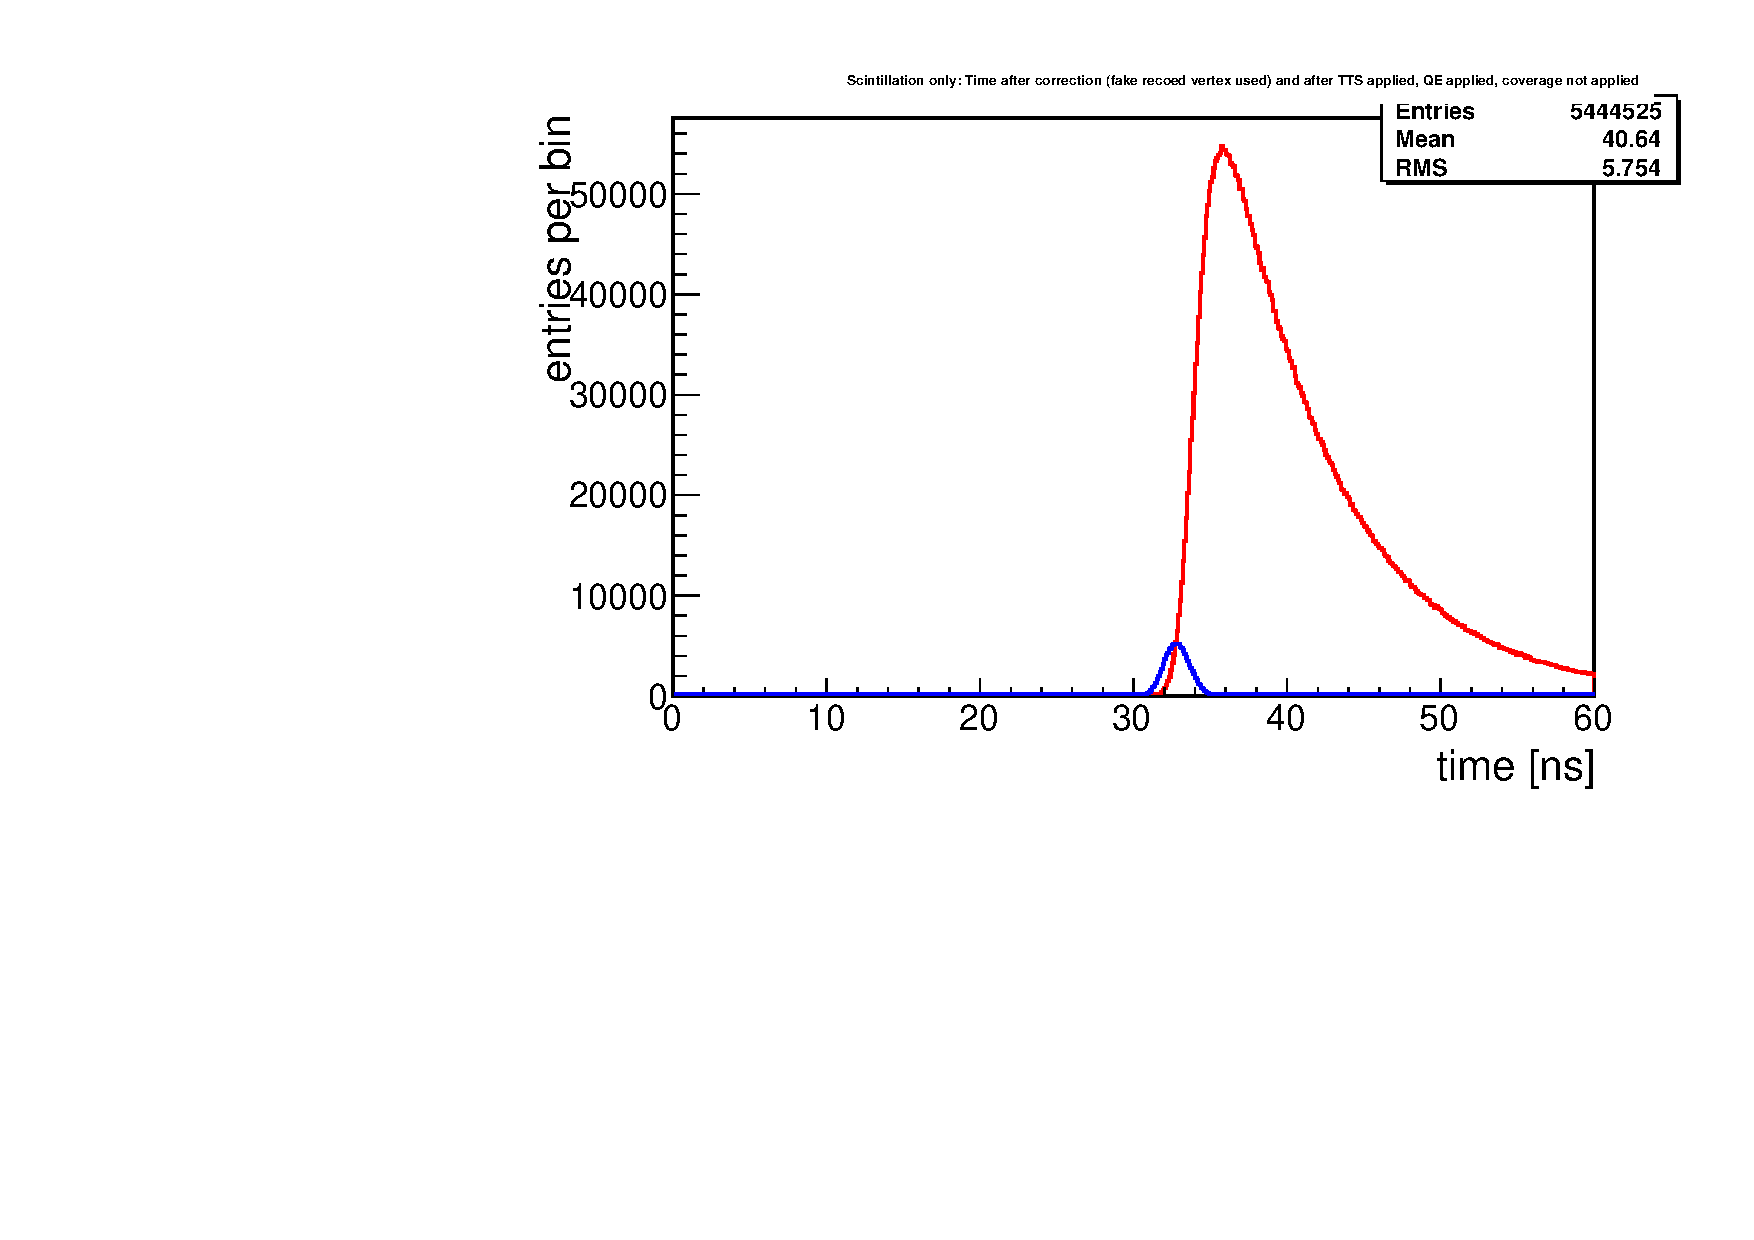
\includegraphics[scale=0.40]{graphs/6p5Meter_5MeVElectrons_Bialkali_KamlandScintSpec_TIME.pdf}
        \caption[]{Effectively reconstructed PE times for the simulation of 1000 electrons (5~MeV) with default settings: Detector diameter = 6.5~m, bialkali photocathode, KamLAND scintillator emission spectrum, TTS = 0.1~ns ($\sigma$). PEs from Cerenkov light only (blue) and scintillation light only (red) are compared. The number of PEs per event after a 33.0~ns time cut is 37 from scintillation and 64 from Cerenkov. \label{6p5Meter_5MeVElectrons_Bialkali_KamlandScintSpec_TIME}}
        \end{center}
\end{figure}
\begin{figure}
        \begin{center}
        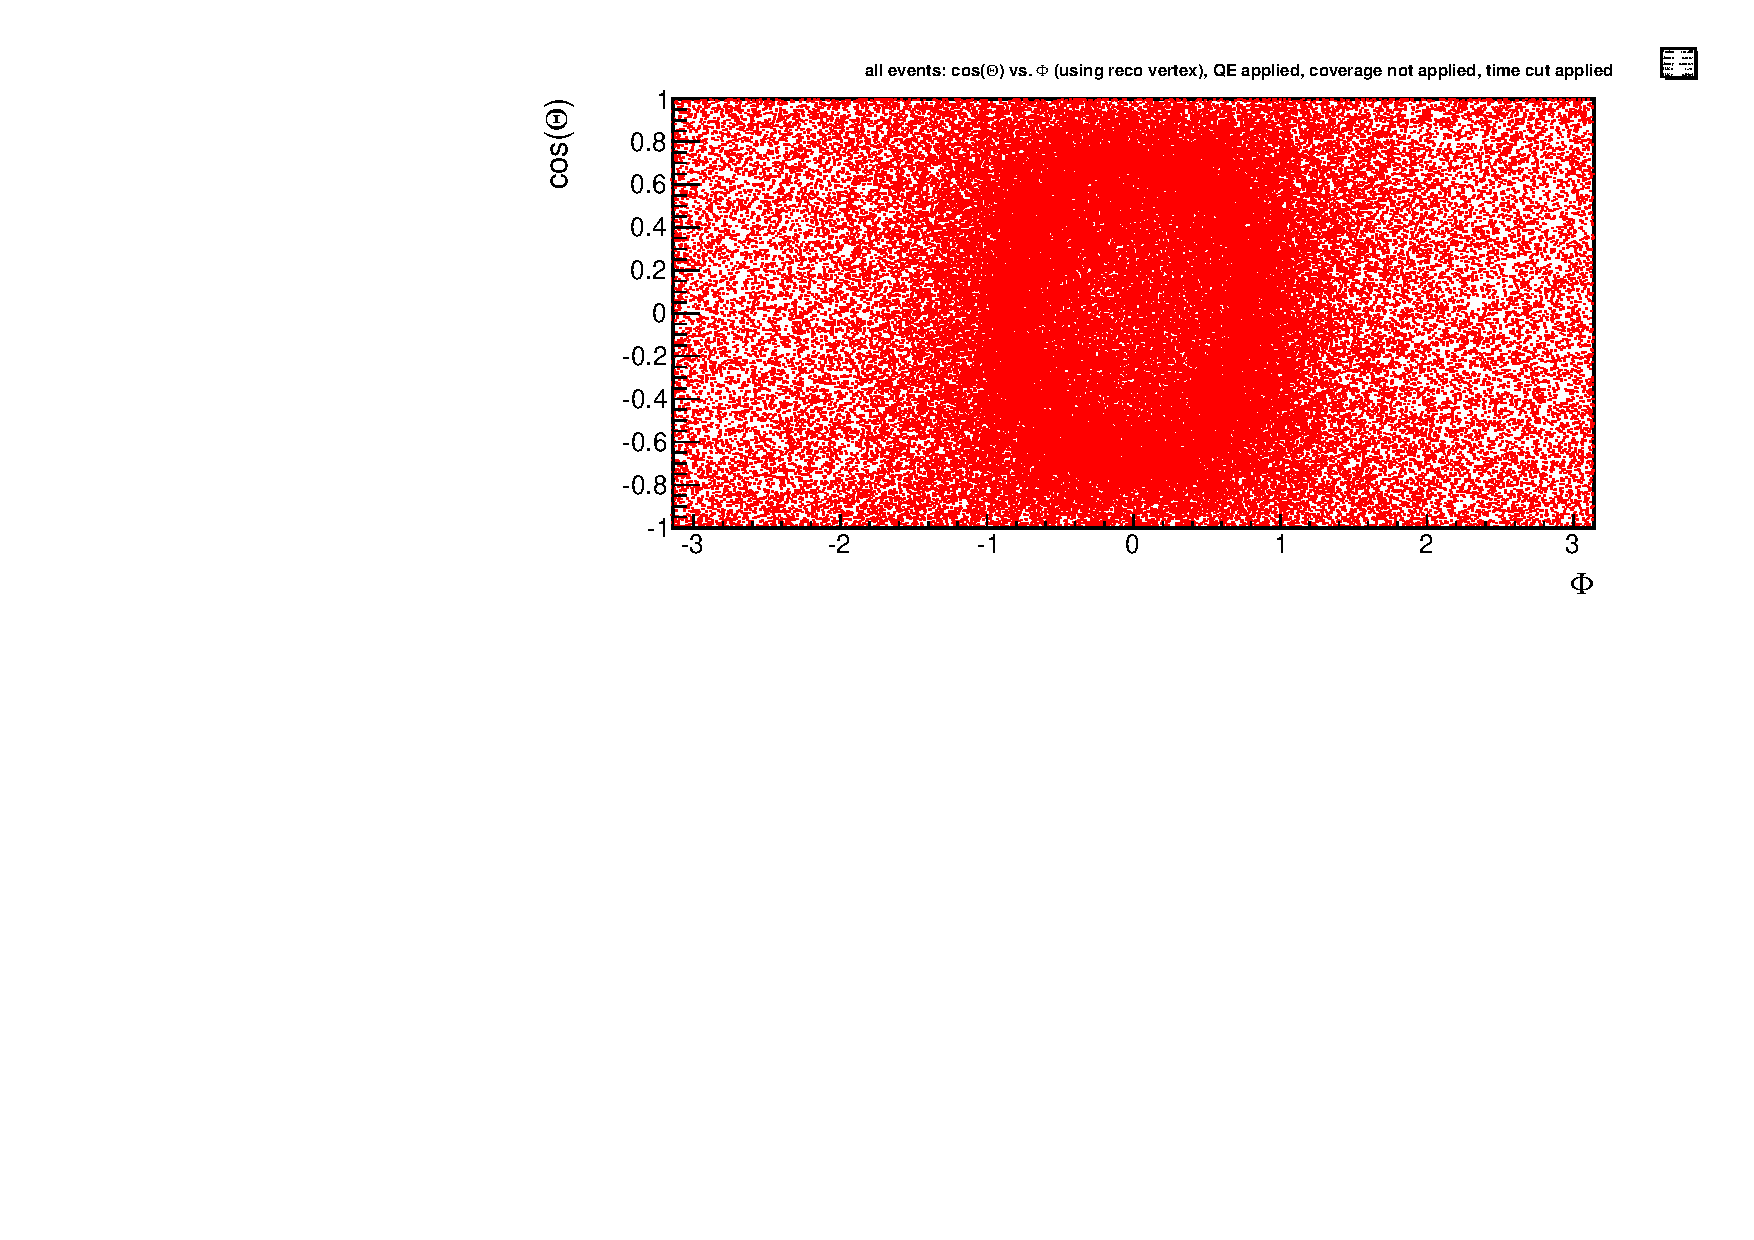
\includegraphics[scale=0.40]{graphs/theta_phi.pdf}
        \caption[]{Photoelectron hit positions for 1000 events (5~MeV electrons in x direction) in the default simulation after the effective position reconstruction effect was included and the 33.0~ns time cut has been applied. The azimuthal angle $\Phi$ is zero in x direction and $\pi/2$ in y direction, while $\cos(\Theta)$ ranges from -1 (-z direction) to 1 (z direction). \label{hitpattern_default}}
        \end{center}
\end{figure}
\begin{figure}
        \begin{center}
        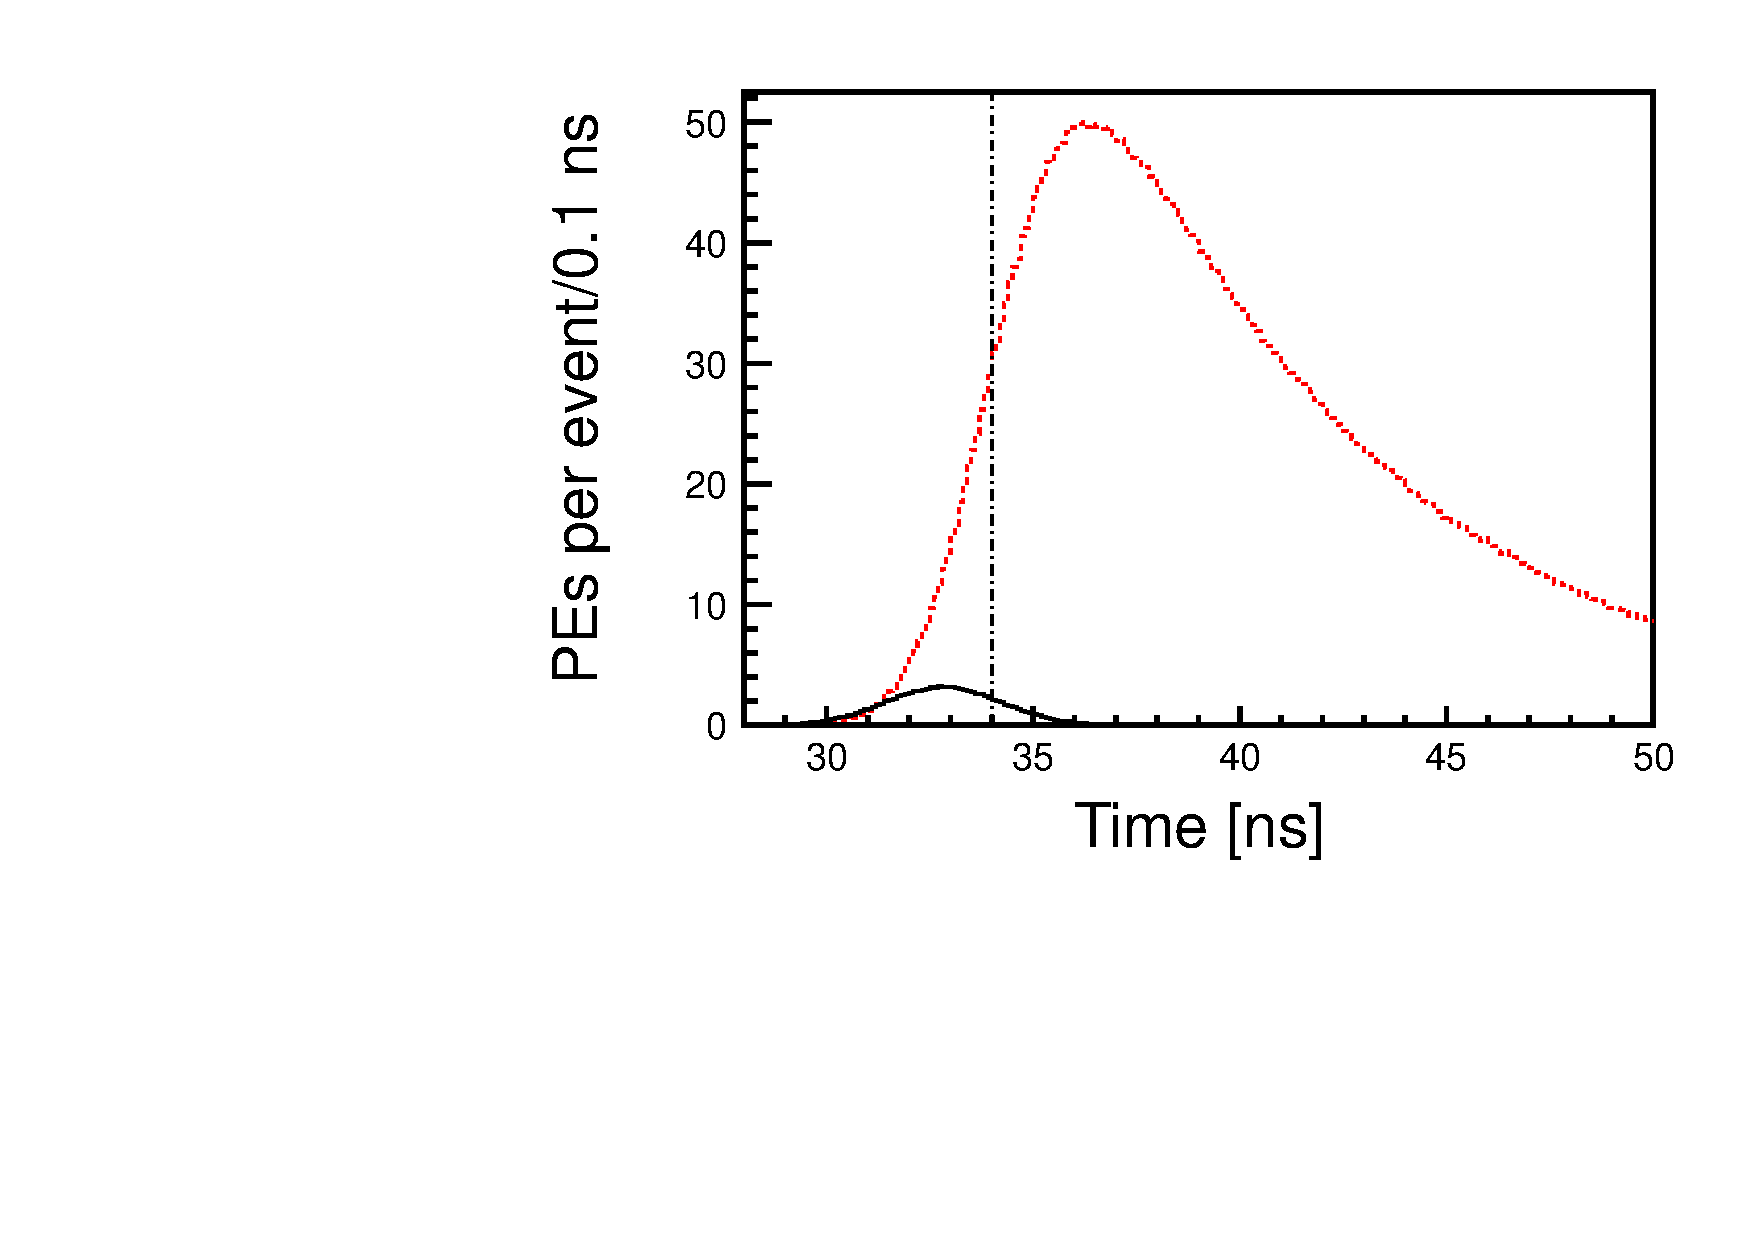
\includegraphics[scale=0.40]{graphs/6p5Meter_5MeVElectrons_Bialkali_KamlandScintSpec_1p28nsTTS_TIME.pdf}
        \caption[]{Effectively reconstructed PE times for the simulation of 1000 electrons (5~MeV) with TTS = 1.28~ns: Detector diameter = 6.5~m, bialkali photocathode, KamLAND scintillator emission spectrum, TTS = 1.28~ns ($\sigma$). PEs from Cerenkov light only (blue) and scintillation light only (red) are compared. The number of PEs per event after a 33.0~ns time cut is 153 from scintillation and 60 from Cerenkov. \label{6p5Meter_5MeVElectrons_Bialkali_KamlandScintSpec_1p28nsTTS_TIME}}
        \end{center}
\end{figure}

The settings of the default simulation are described in the previous section. Figure \ref{6p5Meter_5MeVElectrons_Bialkali_KamlandScintSpec_TIME} shows the TOF corrected photoelectron detection time for 1000 simulated electrons with 5~MeV energy in the center of the detector with initial momentum direction coinciding with the x axis. The photoelectrons induced by Cerenkov light arrive earlier, as expected due to the instantaneous emission and the differences in the photon speed. There is however overlap with the PE time distribution coming from scintillation light. In order to compare simulations with different parameters to each other a fixed time cut $t \leq$ 33.0~ns is done (using the truth information of the electron starting time) instead of a more realistic event-by-event time reconstruction. For the default simulation case, the number of PEs coming from Cerenkov light after the time cut (64) is about 58~\% of the total number of PEs from Cerenkov light (110). For scintillation the number of PEs after the time cut (37) is only 0.68~\% (5445).  

Figure \ref{hitpattern_default} displays the PE hit pattern after the 33.0~ns time cut has been applied (1000 events plotted together). Although the time cut is an oversimplification of actual time reconstruction effects, we can use it to indicate the spatial distribution of hits after timing information has been used to separate Cerenkov and scintillation light. The Cerenkov ring structure can be clearly seen (opening angle between 40\textdegree and 50\textdegree) which demonstrates that the directional signal conveyed by the Cerenkov photons is not erased by scattering of the initial 5~MeV electrons.  

If the 17 inch KamLAND PMTs \cite{tbd} (TTS = 1.28~ns) are used in the simulation, the broadening of the time distributions leads to a strongly decreased ratio of Cerenkov over Scintillation light after the time cut (see FIG. \ref{6p5Meter_5MeVElectrons_Bialkali_KamlandScintSpec_1p28nsTTS_TIME}). This demonstrates that the TTS of the photodetectors is critical for directionality reconstruction. Note that the same KamLAND vertex resolution of 12.0~cm has been used in both cases. For detectors with TTS = 0.1~ns ($\sigma$) this number is pessimistic since faster detectors can improve the vertex resolution accuracy. 

\section{Detector Wavelength Response}
\label{detector_wavelength_response_sec} 
In the previous section we saw that low photodetector TTS is highly benefitial for discrimination between Cerenkov and scintillation light. The second important photodetector parameter is the wavelength-dependent QE. Since Cerenkov photons which passed 6.5~m of scintillator have higher average wavelengths than scintillation photons, a photodetector which is more sensitive at high wavelengths increases not only the absolute number of PEs but also the ratio between Cerenkov- and scintillation-induced PEs. Therefore, a simulation has been run with the QE of an extended red-sensitive GaAsP photocathode (the data has been digitized using Hamamatsu R3809U-63 QE data).

\begin{figure}
        \begin{center}
        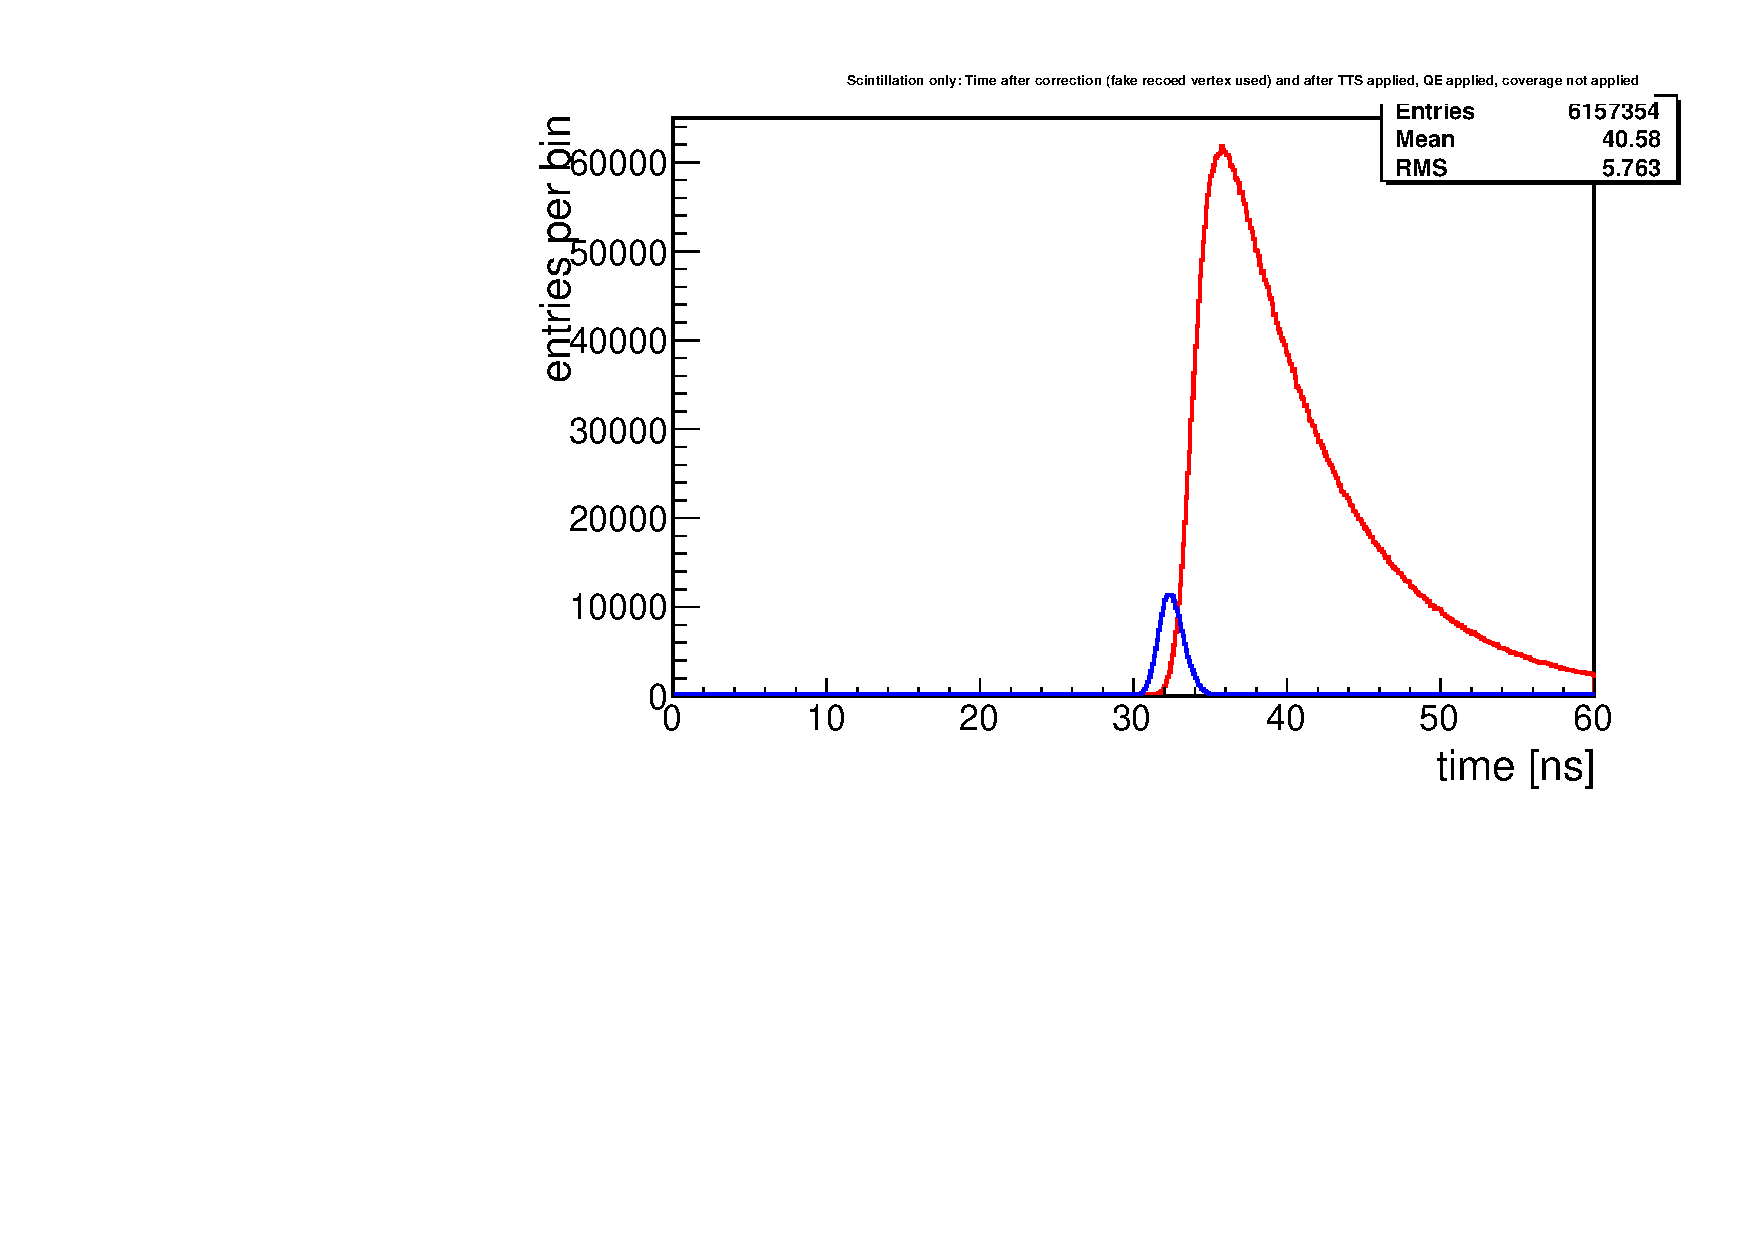
\includegraphics[scale=0.40]{graphs/6p5Meter_5MeVElectrons_RedSensitiveQE_KamlandScintSpec_TIME.pdf}
        \caption[]{Effectively reconstructed PE times for the simulation of 1000 electrons (5~MeV) with red-sensitive photocathode: Detector diameter = 6.5~m, red-sensitive GaAsP photocathode, KamLAND scintillator emission spectrum, TTS = 0.1~ns ($\sigma$). PEs from Cerenkov light only (blue) and scintillation light only (red) are compared. The number of PEs per event after a 33.0~ns time cut is 50.8 from scintillation and 171 from Cerenkov. \label{6p5Meter_5MeVElectrons_RedSensitiveQE_KamlandScintSpec_TIME}}
        \end{center}
\end{figure}

Figure \ref{6p5Meter_5MeVElectrons_RedSensitiveQE_KamlandScintSpec_TIME} shows the results for the modified simulation with high QE in the red spectral region. The higher absolute number of PE coming from Cerenkov light and the increased Cerenkov/scintillation ratio after the time cut (almost doubled compared to the default case) would significantly enhance the directionality reconstruction capabilities.  

\section{Scintillator Emission Spectrum}
\label{scintillator_emission_sec}
One important contributing factor to the separation in time between Cerenkov and scintillation photon hits is the higher average light speed for the photons coming from the Cerenkov effect due to their higher average wavelength. In this section we present two more sets of simulations where the scintillator emission spectrum was changed. 

Recently, the use of quantum dots (QDs) in liquid scintillators has been studied as a possibility to improve future large scale neutrino experiments \cite{tbd}. One important motivation is the control of the emission spectra by tuning the size or composition of the quantum dots. The emission spectrum of alloyed core/shell CdS$_x$Se$_{1-x}$/ZnS Trilite450 \cite{tbd} quantum dots was measured. This spectrum is a symmetric peak centered around 461~nm with FWHM = 29~nm. 

\begin{figure}
        \begin{center}
        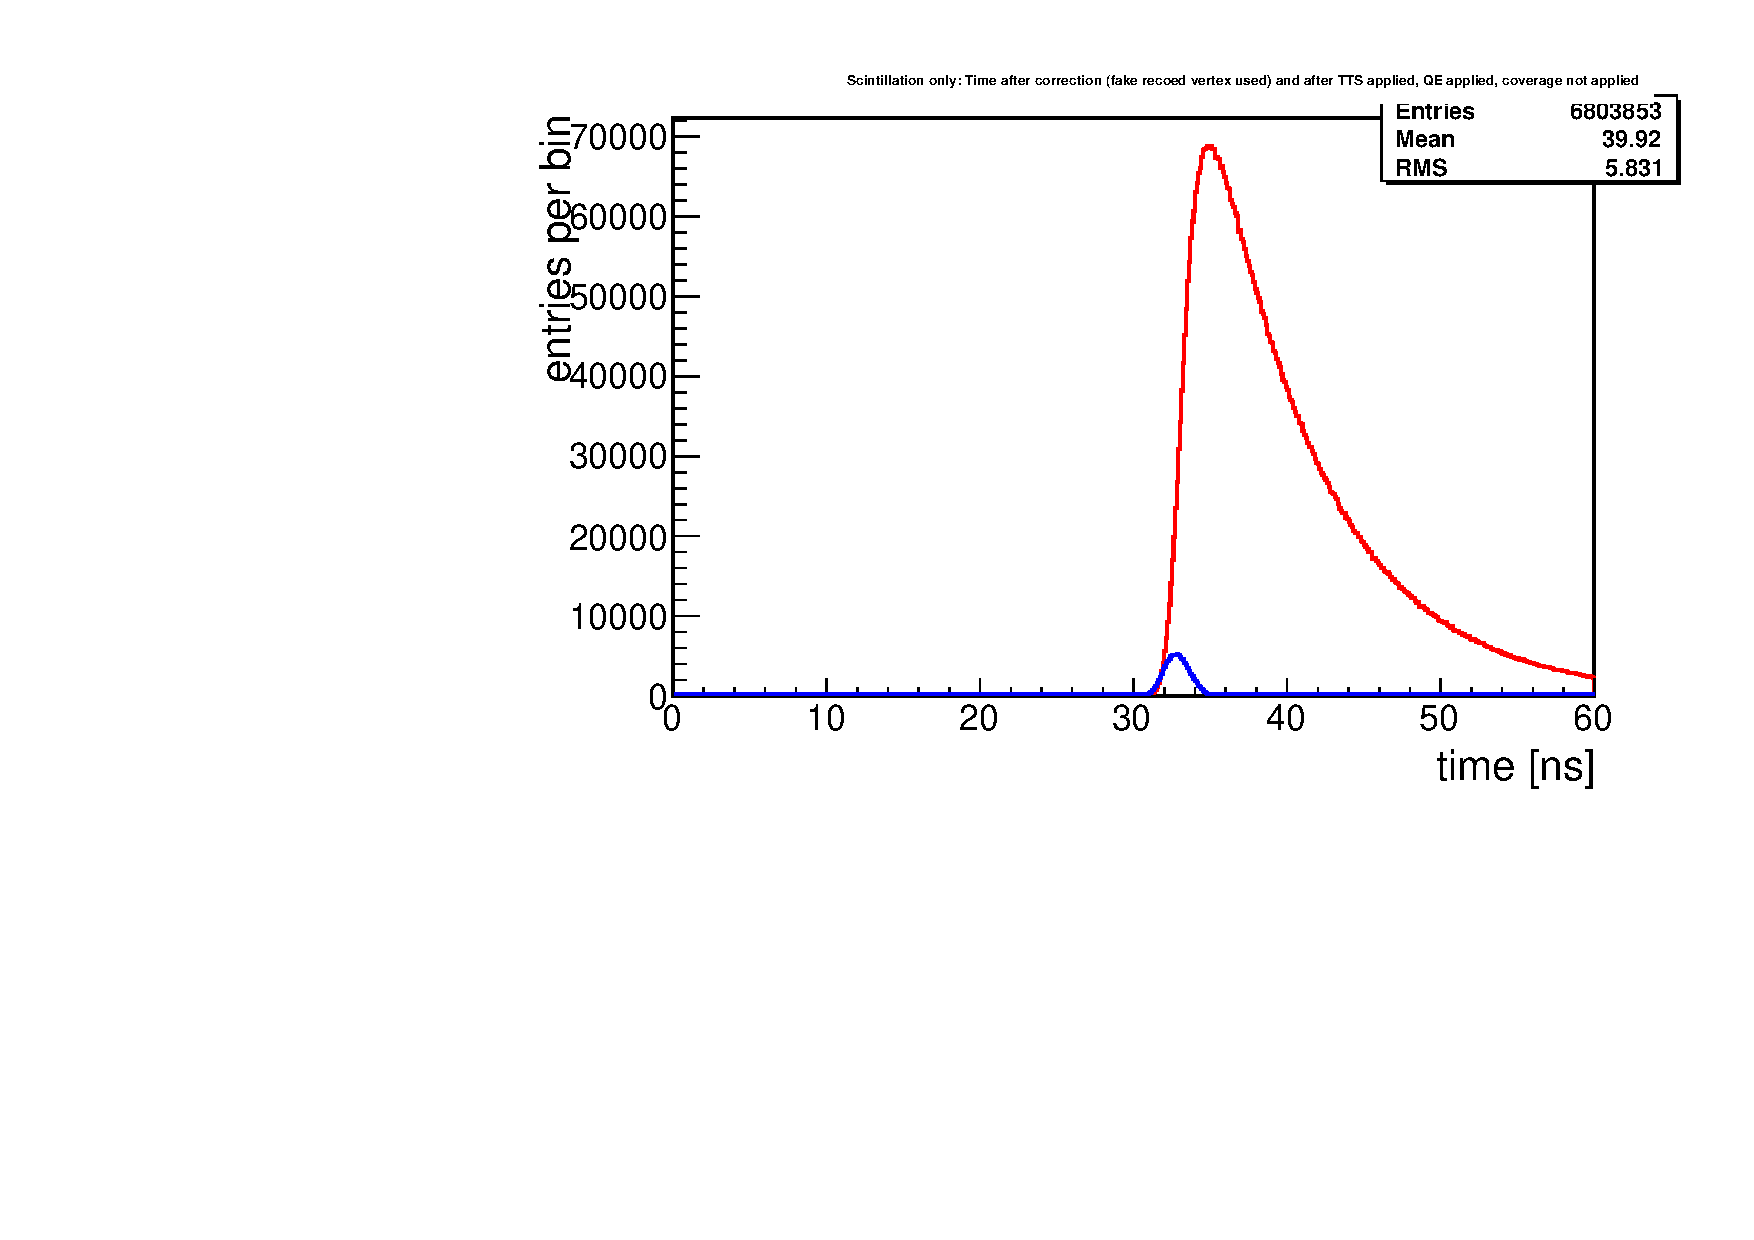
\includegraphics[scale=0.40]{graphs/6p5Meter_5MeVElectrons_Bialkali_QD461nmScintSpec_TIME.pdf}
        \caption[]{Effectively reconstructed PE times for the simulation of 1000 electrons (5~MeV) with QD emission spectrum at 461~nm: Detector diameter = 6.5~m, bialkali photocathode, QD emission spectrum at 461~nm, TTS = 0.1~ns ($\sigma$). PEs from Cerenkov light only (blue) and scintillation light only (red) are compared. The number of PEs per event after a 33.0~ns time cut is 180 from scintillation and 64 from Cerenkov. \label{6p5Meter_5MeVElectrons_Bialkali_QD461nmScintSpec_TIME}}
        \end{center}
\end{figure}  

In order to isolate the effect of a different emission spectrum, the other simulation settings, including the KamLAND absorption spectrum are kept unchanged. In FIG. \ref{6p5Meter_5MeVElectrons_Bialkali_QD461nmScintSpec_TIME} the result for this simulation is presented. Compared to the default case shown in FIG. \ref{6p5Meter_5MeVElectrons_Bialkali_KamlandScintSpec_TIME} the separation is worse because the scintillation light wavelengths are higher than in the KamLAND emission spectrum. However, advances in the production of commercial quantum dot samples could yield quantum dots which have similar, single peak emission shapes at lower wavelengths. This case has been simulated using the same spectral shape of the measured Trilite450 emission but shifted to lower wavelengths such that the emission peak is centered at 384~nm. This peak emission value has been measured for other types of QDs, however with a much more pronounced tail \cite{tbd}. The resulting PE time distribution shows (as expected) a clearer separation of Cerenkov and Scintillation light. After the simple 33.0~ns time cut we obtain slightly better numbers compared to the default simulation: The number of Cerenkov-induced PE after the time cut is unchanged (64) while the number of PEs coming from scintillation light is decreased to 25 (compared to 37 for the default simulation).  

\section{Energy Dependence and Detector Size}
\label{edep_size_sec}
include this? 

The number of Cerenkov photons decreases disproportionally with decreasing electron energy. The number of PEs after the 33~ns time cut for 1~MeV electrons is 8.8 PE from scintillation and 7.7 PE from Cerenkov light. This illustrates that directionality reconstruction benefits from higher initial energies but even at 1~MeV there might be accessible directionality information.  

An additional set of simulations of a 0.65~m diameter ($\approx$ 1~m$^3$) detector with otherwise default parameters was performed. In the smaller detector the chromatic dispersion is not as important and absorption in the scintillator bulk is reduced. The latter effect increases the absolute number of photoelectrons. The former effect, on one hand, reduces the separation in time between Cerenkov and Scintillation light. On the other hand, it reduces the broadening of both time distributions which helps more sophisticated vertex and track reconstruction with the help of fast photodetectors like for example the LAPPDs. However, with the simplified effective vertex reconstruction and a time cut of 3.265~ns we get 87 PEs from scintillation and 87 PEs from Cerenkov. The time cut was adjusted such that the fraction of selected PEs from Cerenkov light matches the fraction in the large detector ($\approx$ 58\%). The QD spectrum discussed in section \ref{scintillator_emission_sec} (both shifted and unshifted) did not change the PE time distribution significantly. We also simulated the red-sensitive photocathode discussed in section \ref{detector_wavelength_response_sec} in the small detector. The amount of PE increases again significantly and with the 3.265~ns time cut the number of PE coming from Cerenkov light is 182 while the number of PE from scintillation light is 96. 

In summary, the photodetector properties (TTS and QE) become more important relative to the scintillator emission and absorption spectra when the detector size is decreased from 6.5~m to 0.65~m.


%%idea: use (some) PMTs with high QE for high lambda (and/or low QE for normal lambda). 
%% add some more info why we are interested in a smaller detector
%% motivation: Daedalus/ISODAR (?), 0nuBB 
\section{Reconstruction}
\label{reconstruction_sec}
Hopefully results

\section{Conclusion}
This is going to work.

\section{Acknowledgements}
Matt, Henry, Janet, Katsushi. Need Andrey's DOE numbers.

\bibliography{DirectionBibliography}

%%20 inch PMTs: 
%%H.~Kume, S.~Sawaki, M.~Ito, K.~Arisaka, T.~Kajita, A.~Nishimura, and A.~Suzuki, Nucl. Instrum. Methods Phys. Res. \bf{205}, 443 (1983).
%%17 inch PMTs: 

\end{document}
